\chapter{支持混合隔离级别机制的\TLAPlus 建模与验证}

\section{事务操作语言的\TLAPlus 表达}
\subsection{状态模型}

第二章已经介绍了 \TLAPlus 与 TLC 的基本概念。本章进一步面向本文提出的事务模型，给出事务操作语言的 \TLAPlus 表达方式。形式化规约仍采用“初始状态 $Init$ + 状态转移 $Next$ + 安全断言”的组织范式，但所有状态变量、动作和约束都围绕混合隔离级别事务的执行过程展开。

在状态建模上，本文将事务执行过程抽象为一个离散状态机。系统状态不仅包含全局键值存储和版本历史，还包含事务缓冲区、事务快照、操作历史以及客户端依赖信息等辅助变量。通过这种建模方式，系统在任意执行时刻的可见状态都能够被形式化描述，为后续的一致性公理检查提供统一语义基础。考虑到完整模块代码篇幅较长，正文仅展示 \url{https://github.com/ZhangJihua0327/mil-tla-verify} 仓库中与建模逻辑直接相关的核心片段。

\begin{figure}[htbp]
    \centering
    \includegraphics[width=0.92\textwidth]{figures/tla-src-code/cut/mixed_isolation_init.pdf}
    \caption{MixedIsolation.tla 中的核心状态变量与初始状态片段}
    \label{fig:tla-init}
\end{figure}

\section{一致性公理和隔离级别约束}

在前文中，我们已经介绍了 \TLAPlus 规约语言及 TLC 模型检查器的基础概念与设计范式。

在本节中，我们将详细阐述如何利用 \TLAPlus 构建一个针对混合隔离级别操作语义的严格验证架构。在此基础上，形式化约束的构造主要包括两部分：其一是将事务执行历史转化为抽象执行中的 $\text{VIS}$ 与 $\text{AR}$ 关系；其二是将一致性公理与隔离级别约束转化为可由 TLC 检查的逻辑断言。
\subsection{状态变量与动作定义}
\subsubsection{状态模型}

定义操作语义的第一步是定义状态模型。我们使用一个状态变量来表示系统的当前状态，这个状态变量可以包含多个组件，例如事务的状态、数据项的值、锁的状态等。通过定义这些组件，我们可以准确地描述系统在任意时刻的状态。

重要的变量有：
\begin{itemize}
    \item \texttt{store}: 全局键值存储，模拟数据库的持久化状态。它是一个映射，键是 Keys，值是版本历史（包含值、提交时间戳 cts、写入者）。
    \item \texttt{tx\_buffer}: 事务的本地写缓冲，模拟事务在提交前对数据的本地修改。
    \item \texttt{tx\_snapshot}: 事务的读取快照版本，决定了事务能看到哪些数据。
    \item \texttt{op\_seq}: 记录操作的历史序列，用于后续的公理化验证。
\end{itemize}

通过以上变量，我们可以构建一个完整的状态模型，准确地描述系统在状态。在这样的基础上，我们可以继续形式化地描述操作语义。

\subsubsection{核心状态转换动作 (Transition Actions)}
操作语义的核心逻辑封装在三个主要的 \TLAPlus  动作定义中：

\textbf{A. 事务开始 ($StartTx(t)$)}

形式化描述了事务如何获取其读取视图（Read View）：
\begin{itemize}
    \item 根据事务的隔离级别 ($Workload[t].level$)，决定 $tx\_snapshot[t]$ 的值。
    \item 例如：SI (Snapshot Isolation) 获取当前的全局 $shard\_ct$（时间戳）。
    \item RA (Read Atomicity) 获取客户端上一次提交的时间 $client\_last\_commit$。
    \item 将事务状态 $tx\_status$ 设为 "Active"。
\end{itemize}

\begin{figure}[htbp]
    \centering
    \includegraphics[width=0.92\textwidth]{figures/tla-src-code/cut/start_tx_rule.pdf}
    \caption{不同隔离级别下的事务启动规则}
    \label{fig:tla-starttx}
\end{figure}

上述片段直接体现了不同隔离级别读取快照的来源差异：PC、SI 和 SER 从全局提交时钟获取一致快照，CC 与 PSI 继承会话依赖，而 RA 仅依赖客户端最近一次提交时间。这一划分将第三章中的语义规则映射为可执行的状态更新条件，也是后续验证 $\text{VIS}$ 构造是否正确的基础。

\textbf{B. 执行操作 ($ExecuteOp(t)$)}

这是读写操作的具体语义描述。它根据 $Workload$ 中预定义的操作类型进行分支：

\begin{enumerate}
    \item \textbf{读操作 ($op.type = "R"$):}
          \begin{itemize}
              \item \textbf{本地优先读取:} 首先检查 $tx\_buffer[t][op.key]$（即写后读 Read-Your-Writes 语义）。
              \item \textbf{快照读取:} 如果本地没有，则调用辅助算子\\ $MaxVersion(store[op.key], tx\_snapshot[t])$。这意味着它会在全局存储的版本历史中，找到提交时间戳小于等于事务快照的最新版本。
              \item \textbf{记录历史:} 将读取结果追加到 $op\_seq$，用于验证。
          \end{itemize}
    \item \textbf{写操作 ($op.type = "W"$):}
          \begin{itemize}
              \item \textbf{写缓冲:} 并不会立即修改全局 $store$，而是更新 $tx\_buffer$。
              \item \textbf{记录历史:} 将写操作追加到 $op\_seq$。
          \end{itemize}
\end{enumerate}

\begin{figure}[htbp]
    \centering
    \includegraphics[width=0.92\textwidth]{figures/tla-src-code/cut/execute_op_rule.pdf}
    \caption{读写操作的核心执行逻辑片段}
    \label{fig:tla-exec}
\end{figure}

该片段保留了两个最关键的语义点。其一，读操作优先检查本地写缓冲，保证事务内部满足 Read-Your-Own-Writes；其二，若本地无写入，则利用 \texttt{MaxVersion} 从满足快照上界的版本集合中选取最新版本。由此，版本可见性被压缩为一个可以由 TLC 直接枚举和检查的选择过程。

\textbf{C. 提交事务 ($CommitTx(t)$)}

形式化描述了提交协议，包括并发控制和原子性：

\begin{enumerate}
    \item \textbf{冲突检测 ($HasConflict$):}
          \begin{itemize}
              \item 定义了谓词 $IsConcurrent(t\_other)$ 来识别并发事务。
              \item 检查是否存在其他并发已提交的事务，其写入集（Writes）与当前事务的检查集（Checkset/ReadSet）有冲突。这对应了乐观并发控制（OCC）的验证阶段。
          \end{itemize}
    \item \textbf{状态更新:}
          \begin{itemize}
              \item \textbf{Abort:} 如果有冲突，状态变为 "Aborted"。
              \item \textbf{Commit:}
                    \begin{itemize}
                        \item 递增全局时间戳 $shard\_ct$。
                        \item \textbf{原子写入:} 将 $tx\_buffer$ 中的数据合并到全局 $store$ 中，生成带有新时间戳的新版本。
                        \item 更新客户端依赖 $client\_dep$。
                    \end{itemize}
          \end{itemize}
\end{enumerate}

\begin{figure}[htbp]
    \centering
    \includegraphics[width=0.92\textwidth]{figures/tla-src-code/cut/commit_tx_rule.pdf}
    \caption{提交阶段中的冲突检测与版本写入片段}
    \label{fig:tla-commit}
\end{figure}

在提交阶段，模型通过 \texttt{HasConflict} 谓词统一表达 PSI、SI 与 SER 等级别所需的并发校验，并在校验通过后以单个状态跃迁完成提交时间分配与新版本写入。由于 \TLAPlus 以状态转移为核心，上述定义能够将“冲突检测”和“原子提交”合并到同一条可验证路径中，从而避免正文中展示与证明无关的工程性细节。

\subsection{抽象执行关系与公理约束}

抽象执行$\mathcal{X} = (\mathcal{H}, \text{VIS}, \text{AR})$，其中 $\mathcal{H}$ 是操作历史，在定义状态模型时，$\mathcal{H}$的内容已经被涉及到，此处不再需要研究，我们需要构建 $\text{VIS}$ 和 $\text{AR}$ 的形式化表达。正文中保留的核心代码图如图~\ref{fig:tla-visar-code} 所示，它直接给出了从已提交事务集合推导 $\text{VIS}$ 与 $\text{AR}$ 的规则。

\begin{figure}[htbp]
    \centering
    \includegraphics[width=0.82\textwidth]{figures/tla-src-code/cut/derived_vis_ar.pdf}
    \caption{从事务提交历史推导 VIS 与 AR 的规则}
    \label{fig:tla-visar-code}
\end{figure}

这里的核心思想是将运行时状态变量直接提升为抽象执行关系。\texttt{Derived\_AR} 使用提交时间戳给出仲裁序，而 \texttt{Derived\_VIS} 则根据事务启动时获得的快照边界或串行化约束生成可见关系。这样，前文定义的一致性公理就不再停留于数学关系层面，而是与模型中的实际状态变量形成一一对应。

现在我们已经定义好抽象执行$\mathcal{X}$，接着我们只需要对公式~\ref{eq:consistency}中的公理进行形式化表达，就可以得到一致性公理的定义。图~\ref{fig:axioms} 展示了公理的形式化表达。通过这些公理，我们就可以定义不同隔离级别的约束。

\begin{figure}[htbp]
    \centering
    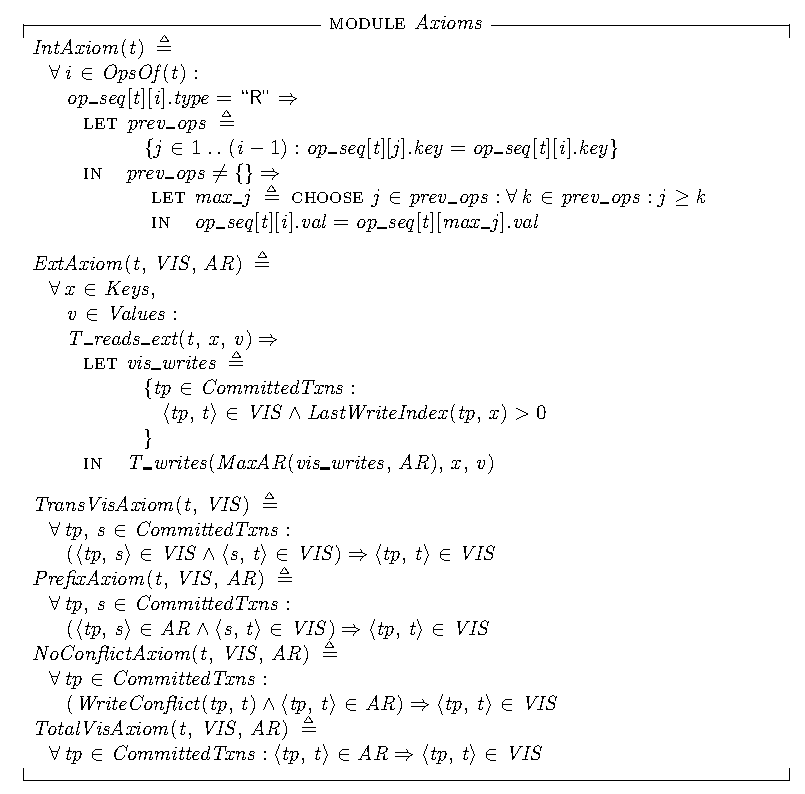
\includegraphics[width=0.75\textwidth]{figures/axioms_cropped.pdf}
    \caption{公理的形式化表达}
    \label{fig:axioms}
\end{figure}

不同于面向具体业务逻辑的程序语言，\TLAPlus 的代码更关注的是状态转移的结果，在运行\TLAPlus 代码时，TLC 模型检查器会穷举所有可能的状态转移路径，并检查在这些路径上是否满足定义的安全属性。通过定义不同的安全属性，我们就可以验证系统在不同隔离级别下是否满足这些属性，从而验证系统的正确性。

\section{模型检查实验与结果}
\subsection{测试方式和测试结果}

测试用例只需通过 \texttt{INSTANCE MixedIsolation WITH ...} 语法注入负载，引擎即可启动运转。在进行验证时，TLC 模型检查器探索所有通过 \texttt{Next} 产生的合法状态转移路径。TLC 的穷举能力确保了网络延迟、乱序提交与快照交错情形都将被覆盖。一旦发现在某个微观并发下，生成的图违反了 \texttt{OperationalSafety == IsConsistentExecution} 断言，就会停止并抛出精准的反例路径追踪报告（Error Trace File），协助开发者定位修缮并发漏洞。

本文在实验阶段采用 SmallBank 负载对混合隔离级别模型进行实例化，原始测试用例如图~\ref{fig:tla-smallbank} 所示。通过注入该负载，TLC 模型检查器能够验证在该负载下系统是否满足定义的安全属性，并且能够发现潜在的并发问题。
通过测试可以看到，在 SmallBank 负载下，系统满足定义的安全属性，并且没有发现潜在的并发问题。这表明在该负载下，系统的操作语义能够保证事务在要求的隔离级别下成立。

\begin{figure}[htbp]
    \centering
    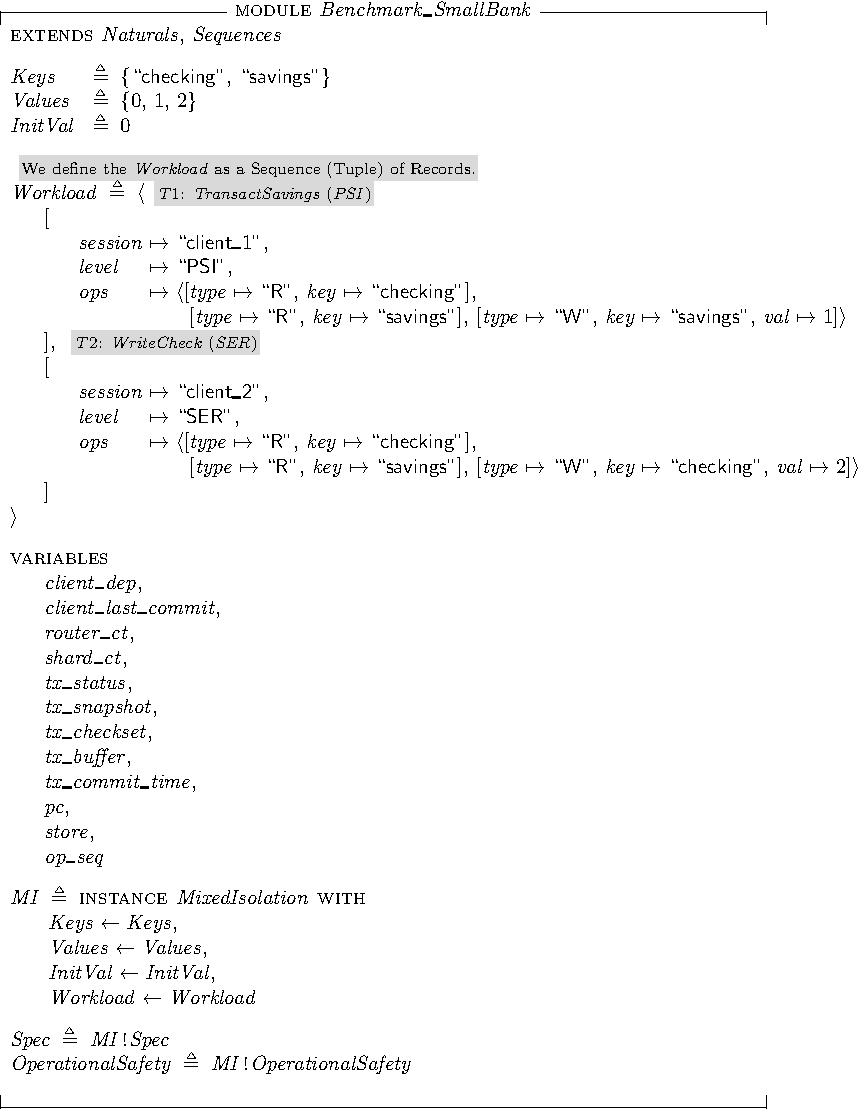
\includegraphics[width=0.92\textwidth]{figures/tla/Benchmark_SmallBank-crop.pdf}
    \caption{SmallBank 负载测试用例}
    \label{fig:tla-smallbank}
\end{figure}

该测试用例给出了一个最小但具有代表性的混合隔离级别验证场景。图中定义了两个并发事务，其中事务 $T_1$ 以 PSI 隔离级别读取 \texttt{checking} 与 \texttt{savings} 两个账户并更新储蓄账户余额，事务 $T_2$ 则以 SER 隔离级别对相同数据项执行读取与写入操作。这样一组负载既保留了 SmallBank 场景中典型的账户读写依赖，又能够显式触发跨事务可见性、检查集冲突以及不同隔离级别交织执行下的一致性约束，因此适合作为 TLC 模型检查的实例化输入。

\begin{figure}[H]
    \centering
    \includegraphics[width=0.9\textwidth]{figures/code/tla_bash.pdf}
    \caption{TLC 模型检查器的终端输出示例}
    \label{fig:tla_bash}
\end{figure}

图~\ref{fig:tla_bash} 展示了 TLC 模型检查器的终端输出示例，其中包含了模型检查的进度、状态生成和发现的状态数量，以及最终的检查结果。通过测试结果可以知道，TLC 模型检查器成功地完成了模型检查，并且没有发现任何违反安全属性的状态。这表明在 SmallBank 负载下，系统的操作语义能够保证事务在要求的隔离级别下成立。

按照同样的方式，我们可以在众多测试集合中进行测试，验证当前操作语义满足定义的安全属性，并且没有发现潜在的并发问题。这表明在这些负载下，系统的操作语义能够保证各类事务在要求的隔离级别下成立。



\section{本章小结}

本章围绕支持混合隔离级别机制的 \TLAPlus 建模与验证展开。首先给出了事务操作语言的 \TLAPlus 表达方式，说明状态变量与核心动作如何共同描述事务执行过程；其次构建了抽象执行关系、一致性公理与隔离级别约束的形式化断言；最后通过模型检查实验与结果分析，验证了本文所设计操作语义能够保证事务在要求的隔离级别下成立，为后续原型系统实现提供了形式化依据。


